\documentclass[../main.tex]{subfiles}

\begin{document}

\section{Architecture}
\label{section:lauxus:architecture}

\begin{figure}[h]
    \centering
    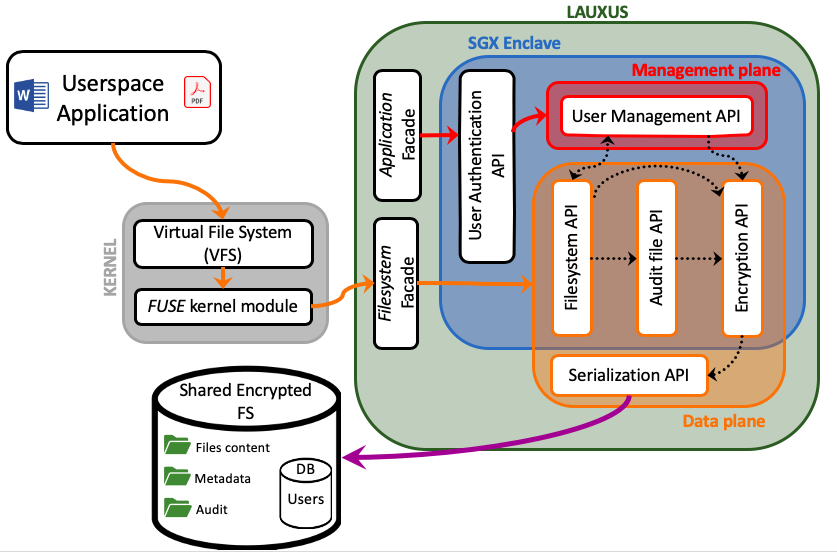
\includegraphics[width=\textwidth]{images/lauxus/architecture}
    
    \caption{Data plane architecture of LAUXUS}
    \label{figure:approach:architecture}
\end{figure}
\par LAUXUS is a software composed of two planes: a data plane and a management plane. The first one is used to simulate a filesystem to which the user-space application interacts. The latter is used to manage the users accessing the filesystem. An illustration of those two planes can be found in Figure \ref{figure:approach:architecture}. In both planes, information is securely stored inside the shared filesystem, in three respective folders: one storing the end-user files, one for the auditing files and a last one for the metadata files. These metadata files enable the filesystem to be shared securely without disclosing information to unauthorised parties.


\subsection{Interaction between planes}
\label{section:lauxus:architecture_process}

\begin{figure}[h]
    \centering
    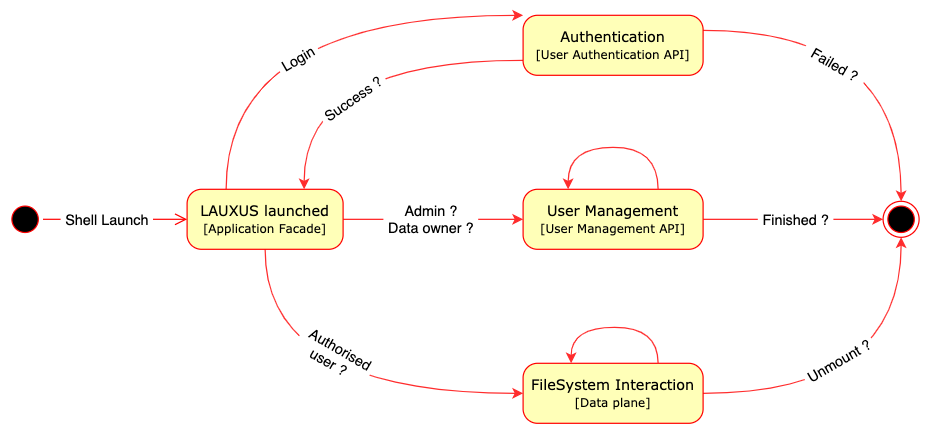
\includegraphics[width=\textwidth]{images/lauxus/architecture_process}
    
    \caption{Interaction between planes}
    \label{figure:lauxus:architecture_process}
\end{figure}
\par In Figure \ref{figure:lauxus:architecture_process} is represented the high-level flow followed by LAUXUS when launched. As we can see, we first go through an authentication process. Second, depending on our role (Administrator / Data owner / Authorised user), we are redirected to either the Management process (with the management plane) or the Filesystem process (with the data plane). Each of these three processes will be covered in details in later sections. First, we will decompose each plane and explain the functionalities of each API presented in Figure \ref{figure:approach:architecture}.


\subsection{Data plane}
\label{section:lauxus:architecture_dataplane}
\par This plane leverages the \textit{FUSE} kernel module to intercept all filesystem operations happening at the kernel level. This allows LAUXUS to be fully transparent for the users and highly increases its portability. The user-space application will interact in the same manner with the Virtual File System as if LAUXUS wasn't even running. In order to communicate with \textit{FUSE} kernel module, we must implement a \textit{Filesystem} facade. The \textit{FUSE} kernel module is composed of a little bit more than 20 endpoints (IO system call) which 15 of them have been implemented in our facade. This means that some filesystem operations will not work but they are not mandatory in order to have a working Filesystem or for running standard filesystem software (e.g: tar, cat, cp, etc). This facade will then interact with the core of our application inside the SGX Enclave which is composed of multiples APIs:
\begin{itemize}
    \item Filesystem API: It is used to simulate a real filesystem and responds to each filesystem operation requested by \textit{FUSE}. It also interacts with the Management Plane for the user entitlement (rights to access a specific file).
    \item Audit File API: It is used to generate and handle audit entries (the purposes of each authorised user action).
    \item Encryption API: It is used to encrypt or decrypt information respectively before saving them to the storage or before using them inside our others API. This layer allows information to be securely handled.
    \item Serialisation API: It is used to interact with the storage (either saving or retrieving information). This layer is outside the Enclave as it no longer handles secret information. Indeed, all the data have been encrypted in the layer before.
\end{itemize}


\subsection{Management plane}
\label{section:lauxus:architecture_mgmntplane}
\par This plane is using an \textit{Application} facade to interact with the core of the application. This facade partially allows the administrator and the owner users to manage the user database (user registration/revocation and/or user entitlement). This facade is also used for the authentication process but will be discussed in Section \ref{section:lauxus:login}. As the data plane, the management plane is composed of multiple APIs:
\begin{itemize}
    \item User Authentication API: It is used to authenticate users into the filesystem. This login will set up a state inside LAUXUS that will be used by the Filesystem API to check the user entitlement.
    \item User Management API: It holds the state of the currently connected user and is used to edit the user database. Interaction with the Users Database is secured with the encryption API.
\end{itemize}

\end{document} 